\section{Theorie}
  \subsection{Das Phasendiagramm}
  \label{sec:phasendiagramm}
  Bei klassischer Betrachtung liegt Wasser in einem der drei Phasen fest, flüssig oder gasförmig vor. In einem geschlossenen Raum eines abgeschlossenen Systems existieren nur
  zwei Freiheitsgrade: der Druck sowie die Temperatur können sich verändern, das Volumen ist fest. Dieser Sachverhalt lässt sich qualitativ darstellen in einem Phasendiagramm:
  \\
  \begin{figure}
    \centering
    \label{fig:phasendiagramm}
      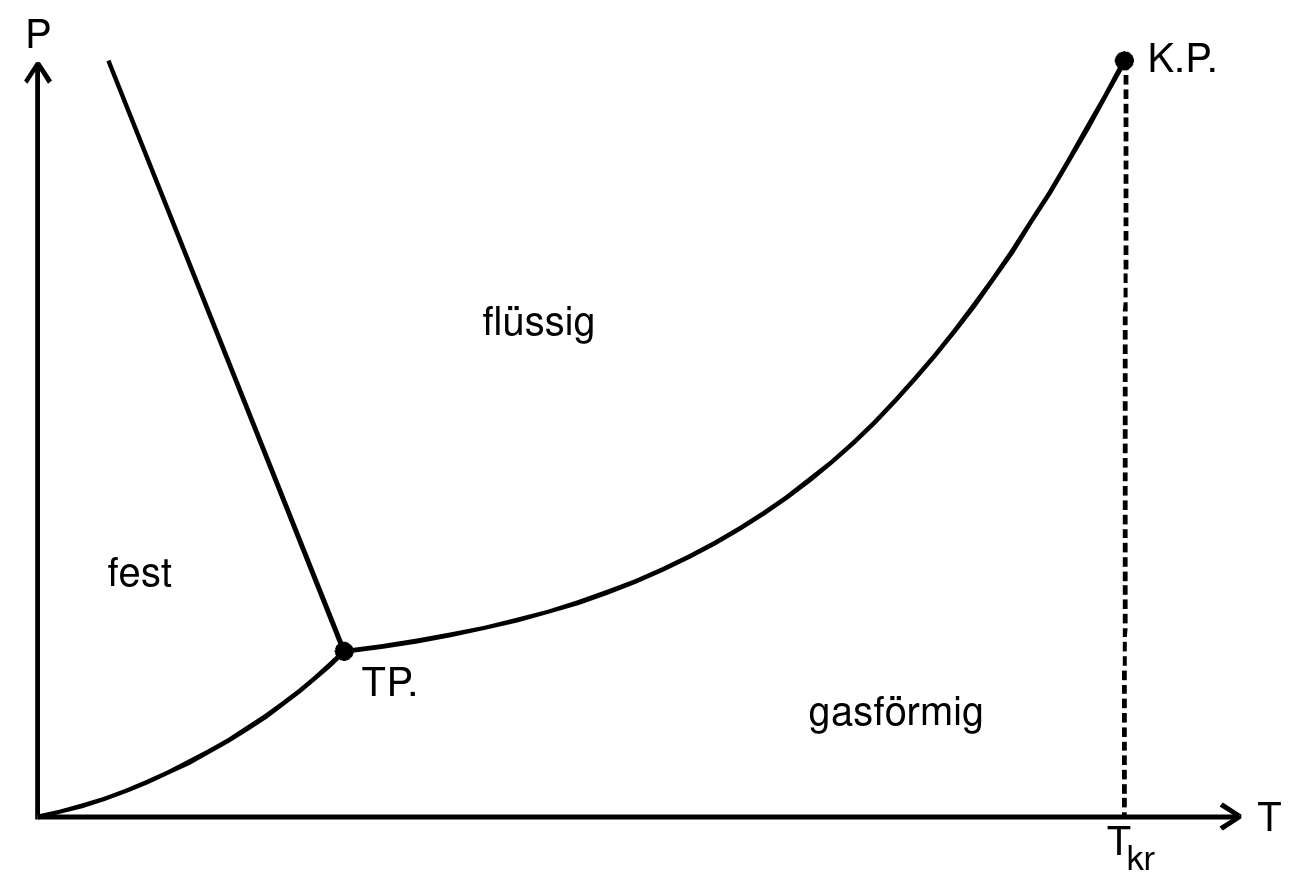
\includegraphics[scale = 0.2]{Content/phasendiagramm.png}
      \caption{ein qualitatives Phasendiagramm für Wasser.}
  \end{figure}
  \\
  \noindent
  Im Folgenden wird der Übergang von flüssig zu gasförmig betrachtet. Die beiden in obiger Abbildung eingezeichneten Punkte TP.
  (Tripelpunkt, hier liegen alle drei Phasen gleichzeitig vor) und K.P. (Kritischer Punkt, hier koexistieren die Phasen flüssig
  und gasförmig nebeneinander)
  begrenzen die Dampfdruckkurve. Der Verlauf dieser Kurve wird bestimmt durch die Größe der Verdampfungswärme $L$, welche für
  jeden Stoff verschieden ist. Sie beschreibt,
  wieviel Wärmeenergie $\increment Q$ nötig ist, um ein mol einer Flüssigkeit zu verdampfen. Diese Größe ist jedoch auch
  temperaturabhängig. Am kritischen Punkt der
  Dampfdruckkurve verschwindet $L$ aufgrund der Koexistenz der flüssigen und gasförmigen Phase, bei den meisten Temperaturen der
  Dampdruckkurve kann die Verdampfungswärme
  aber als näherungsweise konstant angesehen werden.
  \subsection{Die mikroskopischen Vorgänge der Phasenumwandlung}
  \label{sec:mikrovorgänge}
  Wenn in einen abgeschlossenen und evakuierten Raum eine Flüssigkeit gebracht wird, beginnen die Moleküle mit der höchsten
  kinetischen Energie die Flüssigkeit zu verlassen. Dadurch bildet sich oberhalb des Wasserspiegels Dampf. In diesem
  gibt es jedoch auch Moleküle, welche wieder an kinetischer Energie verlieren und in die Flüssigkeit eintauchen. Dies geschieht
  solange, bis sich der Sättigungsdruck einstellt. Dieser ist der Druck, bei welchem genauso viele Moleküle die Flüssigkeit
  verlassen wie wieder in sie zurückkehren. Er ist unabhängig von dem Volumen des Raumes, in dem sich die Flüssigkeit befindet,
  wenn dieses vergrößert oder verkleinert wird, verdampft oder kodensiert eine entsprechende Menge, bis der Sättigungsdruck sich
  wieder eingestellt hat. Daraus folgt, dass sich das System nicht durch die allgemeine Gasgleichung beschreiben lässt:
  \begin{equation}
    \label{eqn:gasgleichung}
      p \cdot V = R_{s} \cdot T
  \end{equation}
  wobei $p$ den Druck, $V$ das Volumen, $R_{S}$ die spezifische Gaskonstante sowie $T$ die Temperatur bezeichnen.
  Der Druck entsteht durch die einzelnen Stöße der Moleküle gegen die Wand des Raumes,
  in welchem sich die Flüssigkeit befindet. Die kinetische Energie der Moleküle wird näherungsweise durch die Maxwellsche
  Geschwindigkeitsverteilung beschrieben. Wenn die Moleküle die Flüssigkeit verlassen, muss Arbeit gegen die Molekularen
  Wechselwirkungen geleistet werden, daher benötigt der Prozess Energie von außen oder sie wird der Flüssigkeit entzogen, diese
  kühlt also ab. Diese Energie ist die Wärmeenergie $\increment Q \si{\joule\per\mol}$. Sie wird bei der Rückkehr der Moleküle in
  die Flüssigkeit, der Kondensation, wieder frei.
  \subsection{Die Dampfdruckkurve}
  \label{sec:dampfdruckkurve}
    Um eine Differentialgleichung zu erhalten, die es ermöglicht, die Dampdruckkurve zu berechnen, beginnt man mit dem
    Kreisprozess der Phasenumwandlung des Wassers im in Abschnitt \ref{sec:mikrovorgänge} Systems.
    \\
    \begin{figure}
      \centering
        \label{fig:kreisprozess}
          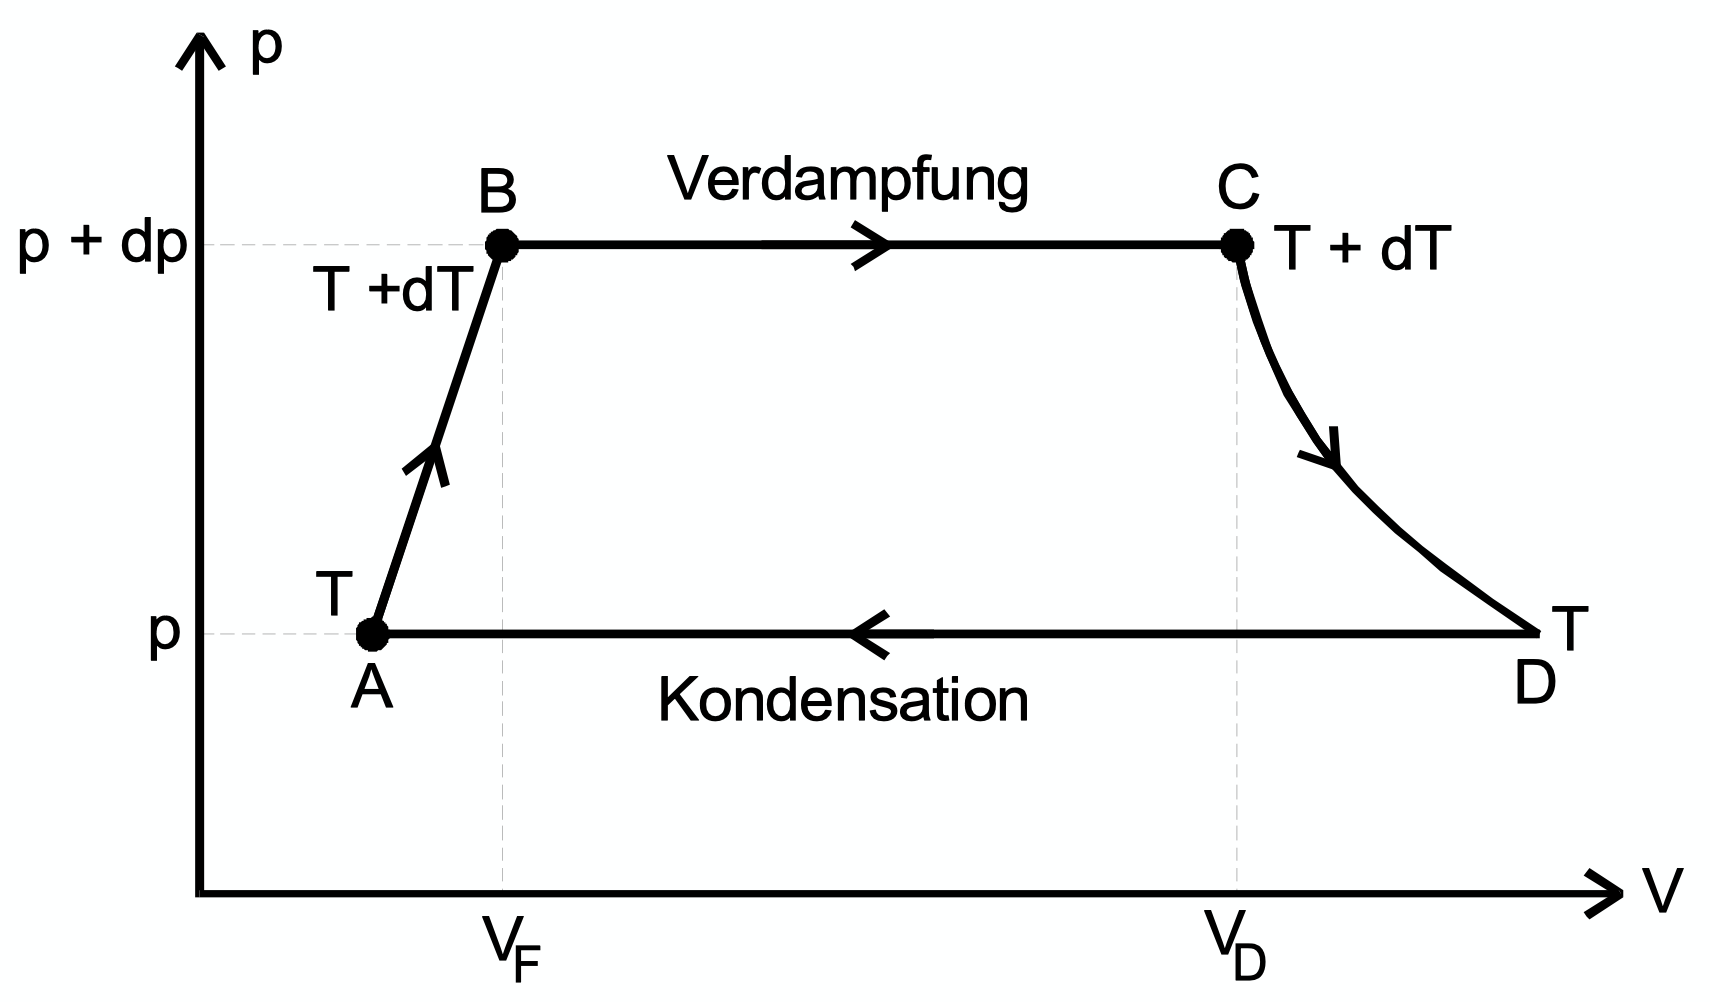
\includegraphics[scale=0.2]{Content/kreisprozess.png}
          \caption{Der Kreisprozess den das Wasser durchläuft, wenn es verdampft und wieder kondensiert.}
    \end{figure}
    \\
    \noindent
    In obiger Grafik ist der Kreisprozess der Verdampfung und Kondensation für ein Mol dargestellt. An Punkt A mit Druck $p$ und
    Temperatur $T$ ist der Stoff flüssig. Nun wird eine Wärmemenge $\increment Q$ hinzugefügt, die Temperatur steigt auf
    $T + \increment T$, der Druck auf $p + \increment p$. Auch das Volumen erhöht sich. Bei Punkt B beginnt der Stoff isobar
    und isotherm zu verdampfen, nur das Volumen ändert sich zu $V_{D}$. An Punkt C sinkt die Temperatur wieder auf $T$ ab, das
    Volumen steigt weiter, während der Druck wieder auf $p$ absinkt. Ab Punkt D gibt der Stoff die Wärmeenergie $\increment Q$
    wieder ab und kondensiert bei gleichbleibender Temperatur und gleichbleibendem Druck. Das Volumen verringert sich auf
    $V_{F}$.
    Wenn man nun über die Energien in diesem Prozess summiert und diese gleich der verrichteten Arbeit gesetzt, erhält man
    \begin{equation*}
      \label{eqn:wärmeenergiearbeit}
      (C_{F} - C_{D})dT + dL = (V_{D} - V_{F})dp.
    \end{equation*}
    Hier bezeichnet $C_{F}$ die Molwärme des flüssigen Stoffes und $C_{D}$ die Molwärme des Dampfes. $dT$ ist die
    Temperaturänderung, $dL$ die benötigte Änderung der Verdampfungswärme und $V_{D}$ sowie $V_{F}$ das Volumen des Dampfes
    respektive der Flüssigkeit. $dP$ bezeichnet die Druckänderung. Nun kann der zweite Hauptsatz der Thermodynamik verwendet
    werden:
    \begin{equation*}
      \label{eqn:zweiterhauptsatz}
      \sum_{i}^{} \frac{Q_{i}}{T_{i}} = 0.
    \end{equation*}
    Wenn man die sich nun ergebende Gleichung ausschreibt, und alle Differentialausdrücke 2. Ordnung vernachlässigt, erhält man
    die Clausius-Clapeyronsche Gleichung
    \begin{equation}
      \label{eqn:clausiusclapeyron}
      (V_{D} - V_{F})dp = \frac{L}{T} dT.
    \end{equation}
    Mit dieser lässt sich prinzipiell die Dampfdruckkurve berechnen, jedoch ist die Integration dieser Differentialgleichung
    potenziell sehr kompliziert, da sowohl $V_{D}$ und $V_{F}$ als auch $L$ komplizierte Funktionen der Temperatur sein können.
    \subsection{Mögliche Vereinfachung der Clausius-Clapeyronschen Gleichung}
    Aufgrund dieser Komplexität wird die Clausius-Clapeyronsche Gleichung im folgenden unter weiter vereinfachenden Annahmen
    gelöst.
    \begin{itemize}
      \item Annahme: $V_{F}$ ist viel kleiner als $V_{D}$ und daher vernachlässigbar.
      \item Annahme: Der Dampf verhält sich näherungsweise wie ein Ideales Gas, $V_{D}$ lässt sich mit dem Idealen-Gas-Gesetz
      berechnen
      \item Annahme: Die Verdampfungswärme $L$ hängt weder vom Druck $p$ noch von der Temperatur $T$ ab
    \end{itemize}
    Unter diesen Vorraussetzungen nimmt Gleichung \eqref{eqn:clausiusclapeyron} die Form
    \begin{equation*}
      \frac{R}{p} dp = \frac{L}{T^{2}} dT
    \end{equation*}
    an. Nun kann integriert werden und es ergibt sich:
    \begin{equation}
      \label{clausiusclapeyronintegriertln}
      \symup{ln}p = - \frac{L}{R} \cdot \frac{1}{T} + const.
    \end{equation}
    Dies kann auch geschrieben werden als
    \begin{equation}
      \label{clausiusclapeyronintegriertexp}
      p = p_{0} exp(- \frac{L}{R} \cdot \frac{1}{T}).
    \end{equation}
\label{sec:Theorie}
